\documentclass[a4paper,10pt]{article}
\nonstopmode
\usepackage{amssymb}
\usepackage{longtable}
\usepackage{ifthen}
\usepackage{pgfplots}
\usepackage[linkcolor=red,pagecolor=red,pdfborder={1 1 1}]{hyperref}
\pgfplotsset{compat=1.4}

\textwidth=16.1cm \textheight=27.0cm \topmargin=-1.8cm
\oddsidemargin=0.1cm \evensidemargin=0.1cm \footskip=45pt

\begin{document}

\pgfplotsset{
/pgfplots/log number format basis/.code 2 args={
  \ifdim #1 pt=2pt
    \ifdim #2 pt>0.5pt
      \ifdim #2 pt<10pt
        \pgfmathparse{#1^#2}
        \pgfmathtruncatemacro\r{\pgfmathresult} \r 
      \else
        \ifdim #2 pt<20pt
          \pgfmathparse{#1^(#2 - 10)}
          \pgfmathprintnumber{\pgfmathresult}K
        \else
          \ifdim #2 pt<30pt
            \pgfmathparse{#1^(#2 - 20)}
            \pgfmathprintnumber{\pgfmathresult}M
          \else
            \ifdim #2 pt<40pt
              \pgfmathparse{#1^(#2 - 30)}
              \pgfmathprintnumber{\pgfmathresult}G
            \else
              \ifdim #2 pt<50pt
                \pgfmathparse{#1^(#2 - 40)}
                \pgfmathprintnumber{\pgfmathresult}T
              \else
                \ifdim #2 pt<60pt
                  \pgfmathparse{#1^(#2 - 50)}
                  \pgfmathprintnumber{\pgfmathresult}P
                \else
                  \ifdim #2 pt<70pt
                    \pgfmathparse{#1^(#2 - 60)}
                    \pgfmathprintnumber{\pgfmathresult}E
                  \else
                    >1Z
                  \fi
                \fi
              \fi
            \fi
          \fi
        \fi
      \fi
    \fi
  \fi
  \ifdim #1 pt=10pt
    $#1^{\pgfmathprintnumber{#2}}$
  \fi
}}

\begin{titlepage}\thispagestyle{empty}
\begin{huge}\begin{flushleft}\bf{OTF Profile}\end{flushleft}\end{huge}
\hrule
\begin{flushright}\textbf{\large Trace Properties}\end{flushright}
\vspace{0.5\baselineskip}
\begin{flushleft}
\begin{tabular}{ll}
\bf{OTF Version:} & \verb|1.12.4salmon| \\
\bf{Creator:} & \verb|VampirTrace 5.14.4|\\
\bf{File:} & \verb|matrix.otf|
\end{tabular}

\vspace{1\baselineskip}
\begin{tabular}{ll}
\bf{Number of Processes:} & \verb|8|\\
\bf{Timer Resolution:} & \verb|2.66683 GHz|
\end{tabular}

\vspace{1\baselineskip}
\begin{tabular}{l}\bf{Comments:}\end{tabular}
\begin{quote}\begin{verbatim}
Trace Times:
 Start: Tue May 19 21:37:07 2015 (1432064227244888)
 Stop: Tue May 19 21:37:11 2015 (1432064231726154)
 Elapsed: 00:00:04 (4481266)
VampirTrace Environment:
 VT_MODE: TRACE
 VT_BUFFER_SIZE: 32M
 VT_SYNC_FLUSH: no
 VT_SYNC_FLUSH_LEVEL: 80
 VT_SNAPSHOTS: yes
 VT_MAX_SNAPSHOTS: 1024
 VT_ONOFF_CHECK_STACK_BALANCE: yes
 VT_MAX_STACK_DEPTH: 0
 VT_MAX_FLUSHES: 1
 VT_METRICS: <not set>
 VT_METRICS_SEP: :
 VT_RUSAGE: <not set>
 VT_MPITRACE: yes
 VT_MPI_IGNORE_FILTER: no
 VT_MEMTRACE: no
 VT_CPUIDTRACE: no
 VT_EXECTRACE: yes
 VT_IOTRACE: no
 VT_IOTRACE_EXTENDED: no
 VT_FILTER_SPEC: <not set>
 VT_GROUPS_SPEC: <not set>
\end{verbatim}\end{quote}
\end{flushleft}
\vspace*{\fill}
\begin{flushright}\today\end{flushright}
\end{titlepage}

\newpage

\begin{center}\small
{\Large \bf Top 27 of 27 Functions}
\bigskip
\begin{longtable}{|l||r|r|r|}

   \hline
   \bf Function & \bf invocations[\#] & \bf excl. time[sec] $\nabla$ & \bf incl. time[sec] \\
   \hline\hline
  \verb|matrix_dot| &   \verb|8| &   \verb|12.7154| &   \verb|15.7655| \\
  \verb|MPI_Init| &   \verb|8| &   \verb|8.30341| &   \verb|8.30529| \\
  \verb|MPI_File_read_all| &   \verb|48| &   \verb|4.3624| &   \verb|4.3624| \\
      \hline
  \verb|MPI_File_write_all| &   \verb|8| &   \verb|3.43061| &   \verb|3.43061| \\
  \verb|MPI_File_close| &   \verb|24| &   \verb|3.12294| &   \verb|3.12294| \\
  \verb|MPI_Sendrecv_replace| &   \verb|112| &   \verb|3.03045| &   \verb|3.03045| \\
      \hline
  \verb|MPI_File_open| &   \verb|24| &   \verb|0.753782| &   \verb|0.753782| \\
  \verb|matrix_read_mpiio| &   \verb|16| &   \verb|0.0434098| &   \verb|6.38499| \\
  \verb|matrix_copy| &   \verb|8| &   \verb|0.0146332| &   \verb|0.0146332| \\
      \hline
  \verb|MPI_File_set_view| &   \verb|24| &   \verb|0.0128555| &   \verb|0.0128555| \\
  \verb|matrix_destroy| &   \verb|32| &   \verb|0.00903565| &   \verb|0.00903565| \\
  \verb|matrix_create| &   \verb|8| &   \verb|0.00487324| &   \verb|0.00487562| \\
      \hline
  \verb|sync time| &   \verb|16| &   \verb|0.00336227| &   \verb|0.00336227| \\
  \verb|MPI_Reduce| &   \verb|16| &   \verb|0.00233633| &   \verb|0.00233633| \\
  \verb|MPI_File_write| &   \verb|2| &   \verb|0.00170034| &   \verb|0.00170034| \\
      \hline
  \verb|main| &   \verb|8| &   \verb|0.000391554| &   \verb|35.8122| \\
  \verb|MPI_Type_create_subarray| &   \verb|24| &   \verb|0.000145314| &   \verb|0.000145314| \\
  \verb|matrix_write_mpiio| &   \verb|8| &   \verb|0.000135831| &   \verb|5.34305| \\
      \hline
  \verb|MPI_Finalize| &   \verb|8| &   \verb|8.53416e-05| &   \verb|0.00156824| \\
  \verb|time_difference| &   \verb|8| &   \verb|6.02227e-05| &   \verb|6.02227e-05| \\
  \verb|create_process_info| &   \verb|8| &   \verb|4.64971e-05| &   \verb|4.64971e-05| \\
      \hline
  \verb|create_partition| &   \verb|24| &   \verb|3.07623e-05| &   \verb|3.07623e-05| \\
  \verb|MPI_Type_commit| &   \verb|24| &   \verb|2.58704e-05| &   \verb|2.58704e-05| \\
  \verb|time_to_double| &   \verb|8| &   \verb|2.00912e-05| &   \verb|2.00912e-05| \\
      \hline
  \verb|MPI_File_seek| &   \verb|1| &   \verb|5.99812e-06| &   \verb|5.99812e-06| \\
  \verb|MPI_Comm_size| &   \verb|8| &   \verb|4.35723e-06| &   \verb|4.35723e-06| \\
  \verb|MPI_Comm_rank| &   \verb|8| &   \verb|2.05187e-06| &   \verb|2.05187e-06| \\
   \hline
\end{longtable}

\end{center}
\newpage

\begin{center}\small
{\Large \bf Top 27 of 27 Functions}
\bigskip
\begin{longtable}{|l||r|r|r|}

   \hline
   \bf Function & \bf invocations[\#] $\nabla$ & \bf excl. time[sec] & \bf incl. time[sec] \\
   \hline\hline
  \verb|MPI_Sendrecv_replace| &   \verb|112| &   \verb|3.03045| &   \verb|3.03045| \\
  \verb|MPI_File_read_all| &   \verb|48| &   \verb|4.3624| &   \verb|4.3624| \\
  \verb|matrix_destroy| &   \verb|32| &   \verb|0.00903565| &   \verb|0.00903565| \\
      \hline
  \verb|create_partition| &   \verb|24| &   \verb|3.07623e-05| &   \verb|3.07623e-05| \\
  \verb|MPI_File_set_view| &   \verb|24| &   \verb|0.0128555| &   \verb|0.0128555| \\
  \verb|MPI_File_close| &   \verb|24| &   \verb|3.12294| &   \verb|3.12294| \\
      \hline
  \verb|MPI_File_open| &   \verb|24| &   \verb|0.753782| &   \verb|0.753782| \\
  \verb|MPI_Type_create_subarray| &   \verb|24| &   \verb|0.000145314| &   \verb|0.000145314| \\
  \verb|MPI_Type_commit| &   \verb|24| &   \verb|2.58704e-05| &   \verb|2.58704e-05| \\
      \hline
  \verb|matrix_read_mpiio| &   \verb|16| &   \verb|0.0434098| &   \verb|6.38499| \\
  \verb|MPI_Reduce| &   \verb|16| &   \verb|0.00233633| &   \verb|0.00233633| \\
  \verb|sync time| &   \verb|16| &   \verb|0.00336227| &   \verb|0.00336227| \\
      \hline
  \verb|time_to_double| &   \verb|8| &   \verb|2.00912e-05| &   \verb|2.00912e-05| \\
  \verb|time_difference| &   \verb|8| &   \verb|6.02227e-05| &   \verb|6.02227e-05| \\
  \verb|matrix_write_mpiio| &   \verb|8| &   \verb|0.000135831| &   \verb|5.34305| \\
      \hline
  \verb|matrix_copy| &   \verb|8| &   \verb|0.0146332| &   \verb|0.0146332| \\
  \verb|matrix_create| &   \verb|8| &   \verb|0.00487324| &   \verb|0.00487562| \\
  \verb|matrix_dot| &   \verb|8| &   \verb|12.7154| &   \verb|15.7655| \\
      \hline
  \verb|create_process_info| &   \verb|8| &   \verb|4.64971e-05| &   \verb|4.64971e-05| \\
  \verb|MPI_File_write_all| &   \verb|8| &   \verb|3.43061| &   \verb|3.43061| \\
  \verb|MPI_Finalize| &   \verb|8| &   \verb|8.53416e-05| &   \verb|0.00156824| \\
      \hline
  \verb|MPI_Comm_size| &   \verb|8| &   \verb|4.35723e-06| &   \verb|4.35723e-06| \\
  \verb|MPI_Comm_rank| &   \verb|8| &   \verb|2.05187e-06| &   \verb|2.05187e-06| \\
  \verb|main| &   \verb|8| &   \verb|0.000391554| &   \verb|35.8122| \\
      \hline
  \verb|MPI_Init| &   \verb|8| &   \verb|8.30341| &   \verb|8.30529| \\
  \verb|MPI_File_write| &   \verb|2| &   \verb|0.00170034| &   \verb|0.00170034| \\
  \verb|MPI_File_seek| &   \verb|1| &   \verb|5.99812e-06| &   \verb|5.99812e-06| \\
   \hline
\end{longtable}

\end{center}
\newpage

\newpage

\begin{flushright}\ttfamily\small
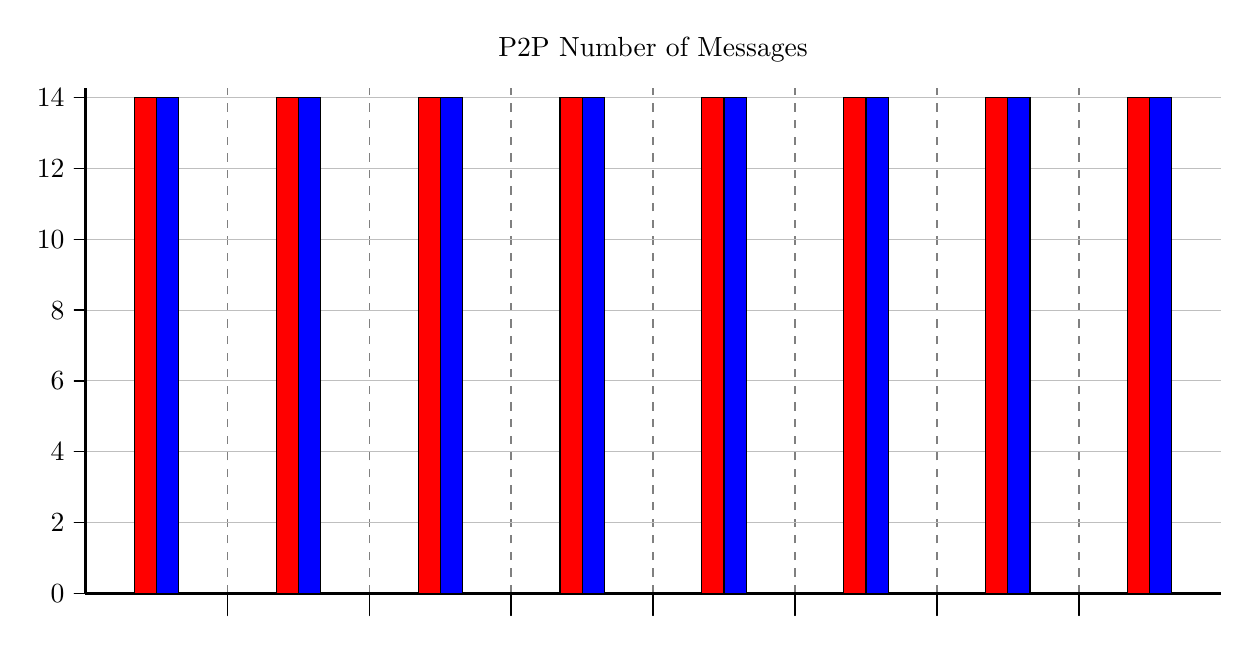
\begin{tikzpicture}
\begin{axis}[
  width=16cm, height=8cm,
  axis x line=bottom,x axis line style={-,line width=1pt},
  axis y line=left,y axis line style={-,line width=1pt},
  enlarge y limits={value=0.02,upper},
  ymin=0,ymajorgrids,xminorgrids,minor x tick num=1,
title=P2P Number of Messages,ylabel={},
x tick label style={rotate=90,anchor=east,font=\ttfamily\footnotesize},
tick align=outside,
tick style={line cap=round,line width=0.5pt,color=black,
      major tick length=4pt,minor tick length=8pt},
major x tick style={line width=1, color=white},
scaled y ticks=true,
bar width=8pt,
minor grid style={color=gray, line width=0.5pt, dashed},
xmin=-0.5,
xmax=7.5,
xtick={0,...,7},
xticklabels={
},]
\addplot[ybar, draw=black, mark=none, fill=red, xshift=-4]
  coordinates{
(0,14)(1,14)(2,14)(3,14)(4,14)(5,14)(6,14)(7,14)};
\addplot[ybar, draw=black, mark=none, fill=blue, xshift=4]
  coordinates{
(0,14)(1,14)(2,14)(3,14)(4,14)(5,14)(6,14)(7,14)};
\end{axis}
\end{tikzpicture}

\end{flushright}
\begin{flushright}\ttfamily\small
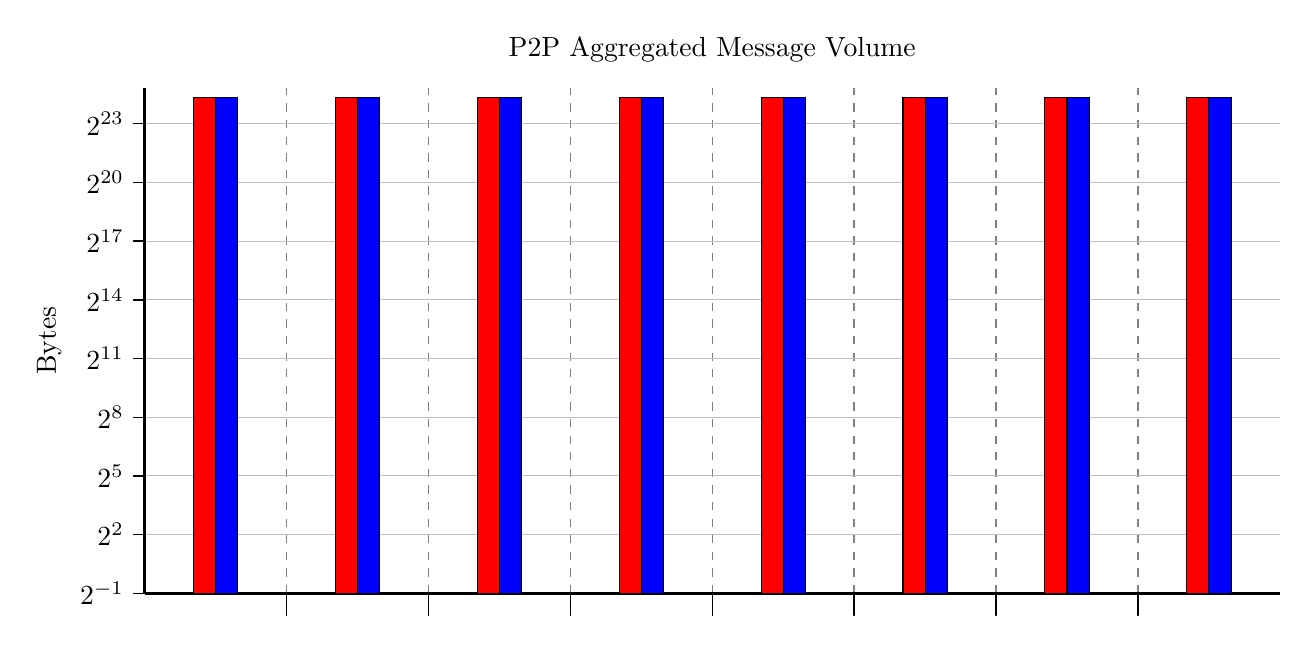
\begin{tikzpicture}
\def \ymin {0.5}
\begin{axis}[
  width=16cm, height=8cm,
  axis x line=bottom,x axis line style={-,line width=1pt},
  axis y line=left,y axis line style={-,line width=1pt},
  enlarge y limits={value=0.02,upper},
  ymode=log,log basis y=2,ymin=\ymin,
  try min ticks log={8},
ymajorgrids,xminorgrids,minor x tick num=1,
title=P2P Aggregated Message Volume,ylabel={Bytes},
x tick label style={rotate=90,anchor=east,font=\ttfamily\footnotesize},
tick align=outside,
tick style={line cap=round,line width=0.5pt,color=black,
      major tick length=4pt,minor tick length=8pt},
major x tick style={line width=1, color=white},
scaled y ticks=true,
bar width=8pt,
minor grid style={color=gray, line width=0.5pt, dashed},
xmin=-0.5,
xmax=7.5,
xtick={0,...,7},
xticklabels={
},]
\addplot[ybar, draw=black, mark=none, fill=red, xshift=-4]
  coordinates{
(0,21000224)(1,21000224)(2,21000224)(3,21000224)(4,21000224)(5,21000224)(6,21000224)(7,21000224)};
\addplot[ybar, draw=black, mark=none, fill=blue, xshift=4]
  coordinates{
(0,21000224)(1,21000224)(2,21000224)(3,21000224)(4,21000224)(5,21000224)(6,21000224)(7,21000224)};
\end{axis}
\end{tikzpicture}

\end{flushright}
\begin{flushright}\ttfamily\small
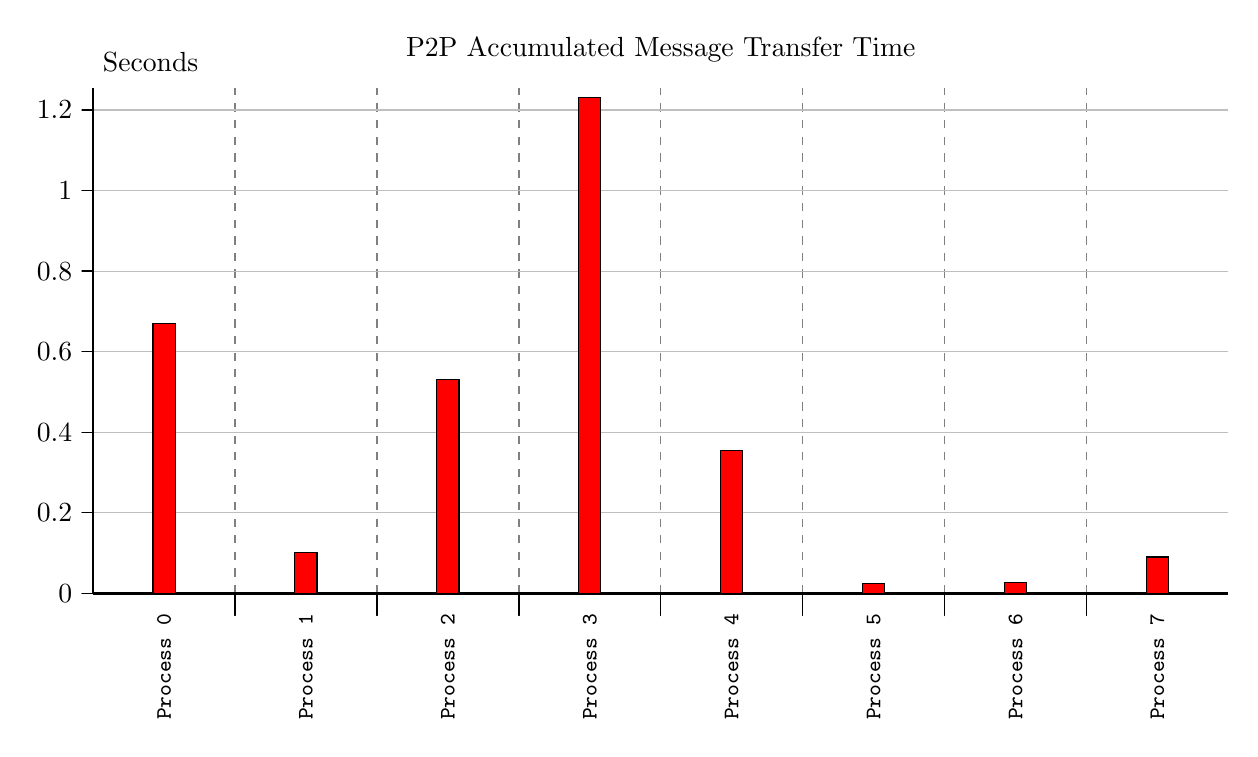
\begin{tikzpicture}
\begin{axis}[
  width=16cm, height=8cm,
  axis x line=bottom,x axis line style={-,line width=1pt},
  axis y line=left,y axis line style={-,line width=1pt},
  enlarge y limits={value=0.02,upper},
ymin=0,
  ylabel style={at={(0,7cm)},rotate=-90,anchor=north west},
ymajorgrids,xminorgrids,minor x tick num=1,
title=P2P Accumulated Message Transfer Time,ylabel={Seconds},
x tick label style={rotate=90,anchor=east,font=\ttfamily\footnotesize},
tick align=outside,
tick style={line cap=round,line width=0.5pt,color=black,
      major tick length=4pt,minor tick length=8pt},
major x tick style={line width=1, color=white},
scaled y ticks=true,
bar width=8pt,
minor grid style={color=gray, line width=0.5pt, dashed},
xmin=-0.5,
xmax=7.5,
xtick={0,...,7},
xticklabels={
Process 0,Process 1,Process 2,Process 3,Process 4,Process 5,Process 6,Process 7,},]
\addplot[ybar, draw=black, mark=none, fill=red]
  coordinates{
(0,0.671019114)(1,0.102208344)(2,0.531067554)(3,1.23044277)(4,0.355556886)(5,0.0242226452)(6,0.0258743761)(7,0.0900575885)};
\end{axis}
\end{tikzpicture}

\end{flushright}
\begin{flushright}
\bigskip

\begin{tikzpicture}
\node(a) at (0,0) [rectangle, draw, fill=red] {};
\node [black,right] at (a.east) {send};
\node(b) at (2,0) [rectangle, draw, fill=blue] {};
\node [black,right] at (b.east) {receive};
\end{tikzpicture}
\end{flushright}
\newpage

\center{\Large \bf P2P - Message Data Rate Histogram}
\bigskip

\begin{center}
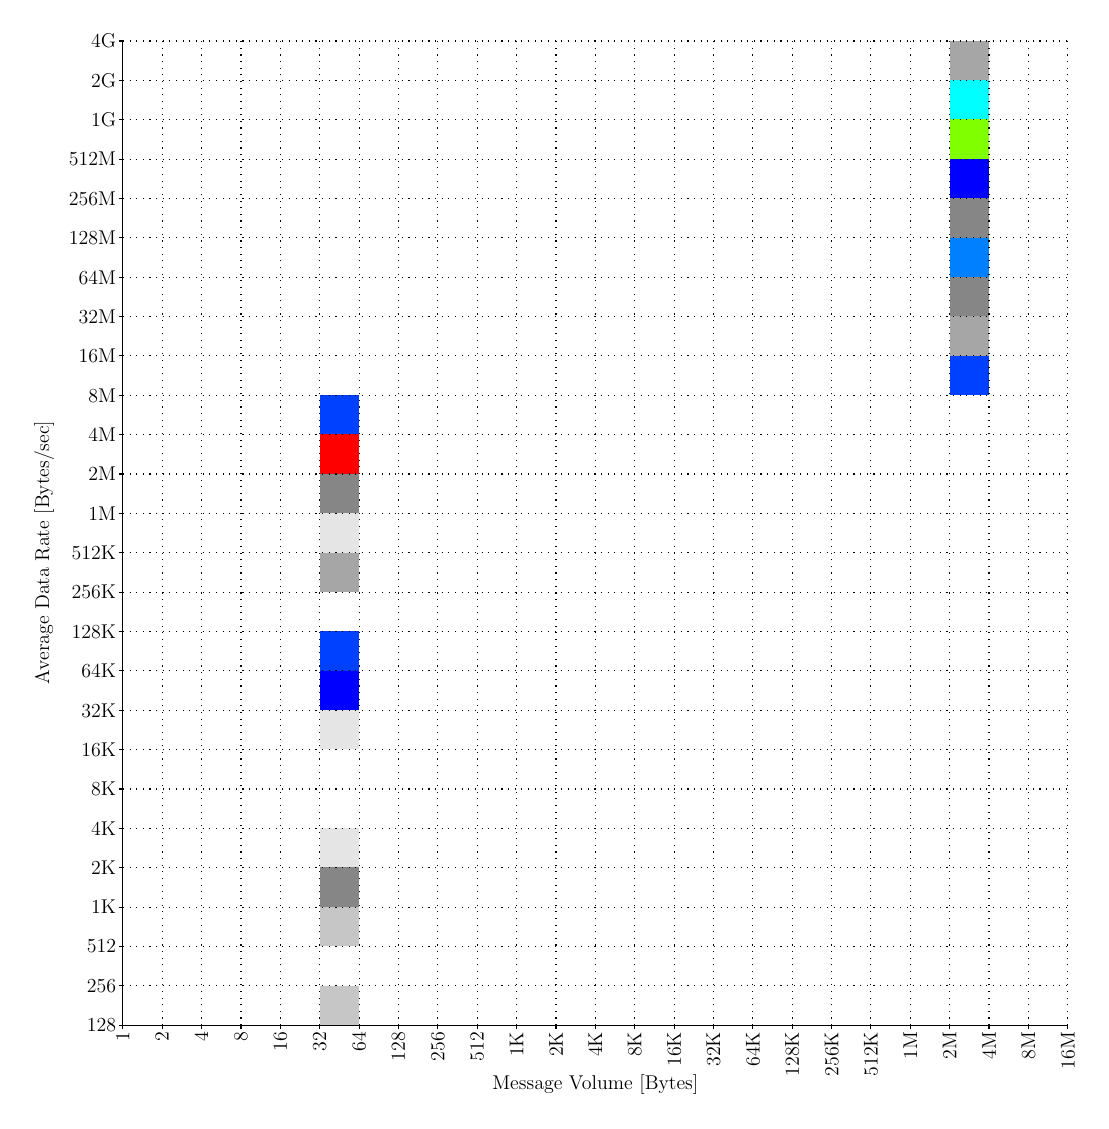
\begin{tikzpicture} [step=1cm,scale=0.5,every node/.style={scale=0.5}]\Large
\node[minimum size=1cm,anchor=south west] at (5,0) [rectangle, fill={rgb,1:red,0.775000;green,0.775000;blue,0.775000}] {};
\node[minimum size=1cm,anchor=south west] at (5,2) [rectangle, fill={rgb,1:red,0.775000;green,0.775000;blue,0.775000}] {};
\node[minimum size=1cm,anchor=south west] at (5,3) [rectangle, fill={rgb,1:red,0.525000;green,0.525000;blue,0.525000}] {};
\node[minimum size=1cm,anchor=south west] at (5,4) [rectangle, fill={rgb,1:red,0.900000;green,0.900000;blue,0.900000}] {};
\node[minimum size=1cm,anchor=south west] at (5,7) [rectangle, fill={rgb,1:red,0.900000;green,0.900000;blue,0.900000}] {};
\node[minimum size=1cm,anchor=south west] at (5,8) [rectangle, fill={rgb,1:red,0.000000;green,0.000000;blue,1.000000}] {};
\node[minimum size=1cm,anchor=south west] at (5,9) [rectangle, fill={rgb,1:red,0.000000;green,0.250000;blue,1.000000}] {};
\node[minimum size=1cm,anchor=south west] at (5,11) [rectangle, fill={rgb,1:red,0.650000;green,0.650000;blue,0.650000}] {};
\node[minimum size=1cm,anchor=south west] at (5,12) [rectangle, fill={rgb,1:red,0.900000;green,0.900000;blue,0.900000}] {};
\node[minimum size=1cm,anchor=south west] at (5,13) [rectangle, fill={rgb,1:red,0.525000;green,0.525000;blue,0.525000}] {};
\node[minimum size=1cm,anchor=south west] at (5,14) [rectangle, fill={rgb,1:red,1.000000;green,0.000000;blue,0.000000}] {};
\node[minimum size=1cm,anchor=south west] at (5,15) [rectangle, fill={rgb,1:red,0.000000;green,0.250000;blue,1.000000}] {};
\node[minimum size=1cm,anchor=south west] at (21,16) [rectangle, fill={rgb,1:red,0.000000;green,0.250000;blue,1.000000}] {};
\node[minimum size=1cm,anchor=south west] at (21,17) [rectangle, fill={rgb,1:red,0.650000;green,0.650000;blue,0.650000}] {};
\node[minimum size=1cm,anchor=south west] at (21,18) [rectangle, fill={rgb,1:red,0.525000;green,0.525000;blue,0.525000}] {};
\node[minimum size=1cm,anchor=south west] at (21,19) [rectangle, fill={rgb,1:red,0.000000;green,0.500000;blue,1.000000}] {};
\node[minimum size=1cm,anchor=south west] at (21,20) [rectangle, fill={rgb,1:red,0.525000;green,0.525000;blue,0.525000}] {};
\node[minimum size=1cm,anchor=south west] at (21,21) [rectangle, fill={rgb,1:red,0.000000;green,0.000000;blue,1.000000}] {};
\node[minimum size=1cm,anchor=south west] at (21,22) [rectangle, fill={rgb,1:red,0.500000;green,1.000000;blue,0.000000}] {};
\node[minimum size=1cm,anchor=south west] at (21,23) [rectangle, fill={rgb,1:red,0.000000;green,1.000000;blue,1.000000}] {};
\node[minimum size=1cm,anchor=south west] at (21,24) [rectangle, fill={rgb,1:red,0.650000;green,0.650000;blue,0.650000}] {};
\draw (0,-0.1) -- (0,0) node[rotate=90,left] at (0,0) {1};
\draw (1,-0.1) -- (1,0) node[rotate=90,left] at (1,0) {2};
\draw (2,-0.1) -- (2,0) node[rotate=90,left] at (2,0) {4};
\draw (3,-0.1) -- (3,0) node[rotate=90,left] at (3,0) {8};
\draw (4,-0.1) -- (4,0) node[rotate=90,left] at (4,0) {16};
\draw (5,-0.1) -- (5,0) node[rotate=90,left] at (5,0) {32};
\draw (6,-0.1) -- (6,0) node[rotate=90,left] at (6,0) {64};
\draw (7,-0.1) -- (7,0) node[rotate=90,left] at (7,0) {128};
\draw (8,-0.1) -- (8,0) node[rotate=90,left] at (8,0) {256};
\draw (9,-0.1) -- (9,0) node[rotate=90,left] at (9,0) {512};
\draw (10,-0.1) -- (10,0) node[rotate=90,left] at (10,0) {1K};
\draw (11,-0.1) -- (11,0) node[rotate=90,left] at (11,0) {2K};
\draw (12,-0.1) -- (12,0) node[rotate=90,left] at (12,0) {4K};
\draw (13,-0.1) -- (13,0) node[rotate=90,left] at (13,0) {8K};
\draw (14,-0.1) -- (14,0) node[rotate=90,left] at (14,0) {16K};
\draw (15,-0.1) -- (15,0) node[rotate=90,left] at (15,0) {32K};
\draw (16,-0.1) -- (16,0) node[rotate=90,left] at (16,0) {64K};
\draw (17,-0.1) -- (17,0) node[rotate=90,left] at (17,0) {128K};
\draw (18,-0.1) -- (18,0) node[rotate=90,left] at (18,0) {256K};
\draw (19,-0.1) -- (19,0) node[rotate=90,left] at (19,0) {512K};
\draw (20,-0.1) -- (20,0) node[rotate=90,left] at (20,0) {1M};
\draw (21,-0.1) -- (21,0) node[rotate=90,left] at (21,0) {2M};
\draw (22,-0.1) -- (22,0) node[rotate=90,left] at (22,0) {4M};
\draw (23,-0.1) -- (23,0) node[rotate=90,left] at (23,0) {8M};
\draw (24,-0.1) -- (24,0) node[rotate=90,left] at (24,0) {16M};
\draw (-0.1,0) -- (0,0) node[anchor=east] at (0,0) {128};
\draw (-0.1,1) -- (0,1) node[anchor=east] at (0,1) {256};
\draw (-0.1,2) -- (0,2) node[anchor=east] at (0,2) {512};
\draw (-0.1,3) -- (0,3) node[anchor=east] at (0,3) {1K};
\draw (-0.1,4) -- (0,4) node[anchor=east] at (0,4) {2K};
\draw (-0.1,5) -- (0,5) node[anchor=east] at (0,5) {4K};
\draw (-0.1,6) -- (0,6) node[anchor=east] at (0,6) {8K};
\draw (-0.1,7) -- (0,7) node[anchor=east] at (0,7) {16K};
\draw (-0.1,8) -- (0,8) node[anchor=east] at (0,8) {32K};
\draw (-0.1,9) -- (0,9) node[anchor=east] at (0,9) {64K};
\draw (-0.1,10) -- (0,10) node[anchor=east] at (0,10) {128K};
\draw (-0.1,11) -- (0,11) node[anchor=east] at (0,11) {256K};
\draw (-0.1,12) -- (0,12) node[anchor=east] at (0,12) {512K};
\draw (-0.1,13) -- (0,13) node[anchor=east] at (0,13) {1M};
\draw (-0.1,14) -- (0,14) node[anchor=east] at (0,14) {2M};
\draw (-0.1,15) -- (0,15) node[anchor=east] at (0,15) {4M};
\draw (-0.1,16) -- (0,16) node[anchor=east] at (0,16) {8M};
\draw (-0.1,17) -- (0,17) node[anchor=east] at (0,17) {16M};
\draw (-0.1,18) -- (0,18) node[anchor=east] at (0,18) {32M};
\draw (-0.1,19) -- (0,19) node[anchor=east] at (0,19) {64M};
\draw (-0.1,20) -- (0,20) node[anchor=east] at (0,20) {128M};
\draw (-0.1,21) -- (0,21) node[anchor=east] at (0,21) {256M};
\draw (-0.1,22) -- (0,22) node[anchor=east] at (0,22) {512M};
\draw (-0.1,23) -- (0,23) node[anchor=east] at (0,23) {1G};
\draw (-0.1,24) -- (0,24) node[anchor=east] at (0,24) {2G};
\draw (-0.1,25) -- (0,25) node[anchor=east] at (0,25) {4G};
\draw (-0.1,0) -- (24,0);
\draw (0,-0.1) -- (0,25); %y axis
\draw[dotted] (0,0) grid (24,25);
\node[rotate=90] at (-2,12) {Average Data Rate [Bytes/sec]};
\node at (12, -1.5) {Message Volume [Bytes]};
\end{tikzpicture}\bigskip

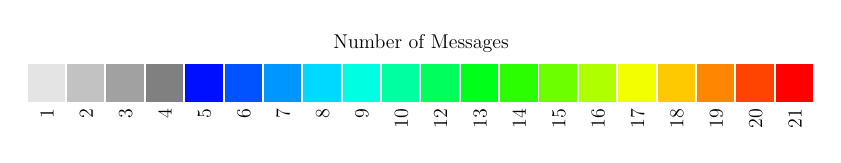
\begin{tikzpicture} [step=1cm,scale=0.5,every node/.style={scale=0.5}]\Large
\node at (11, 0) {Number of Messages};
\node[minimum size=0.95cm,anchor=south west] at (1,-1.5) [rectangle, fill={rgb,1:red,0.893750 ;green,0.893750;blue,0.893750}] {};
\node[anchor=east,rotate=90] at (1.500000,-1.5) {1};
\node[minimum size=0.95cm,anchor=south west] at (2,-1.5) [rectangle, fill={rgb,1:red,0.762500 ;green,0.762500;blue,0.762500}] {};
\node[anchor=east,rotate=90] at (2.500000,-1.5) {2};
\node[minimum size=0.95cm,anchor=south west] at (3,-1.5) [rectangle, fill={rgb,1:red,0.631250 ;green,0.631250;blue,0.631250}] {};
\node[anchor=east,rotate=90] at (3.500000,-1.5) {3};
\node[minimum size=0.95cm,anchor=south west] at (4,-1.5) [rectangle, fill={rgb,1:red,0.500000 ;green,0.500000;blue,0.500000}] {};
\node[anchor=east,rotate=90] at (4.500000,-1.5) {4};
\node[minimum size=0.95cm,anchor=south west] at (5,-1.5) [rectangle, fill={rgb,1:red,0.000000 ;green,0.062500;blue,1.000000}] {};
\node[anchor=east,rotate=90] at (5.500000,-1.5) {5};
\node[minimum size=0.95cm,anchor=south west] at (6,-1.5) [rectangle, fill={rgb,1:red,0.000000 ;green,0.325000;blue,1.000000}] {};
\node[anchor=east,rotate=90] at (6.500000,-1.5) {6};
\node[minimum size=0.95cm,anchor=south west] at (7,-1.5) [rectangle, fill={rgb,1:red,0.000000 ;green,0.587500;blue,1.000000}] {};
\node[anchor=east,rotate=90] at (7.500000,-1.5) {7};
\node[minimum size=0.95cm,anchor=south west] at (8,-1.5) [rectangle, fill={rgb,1:red,0.000000 ;green,0.850000;blue,1.000000}] {};
\node[anchor=east,rotate=90] at (8.500000,-1.5) {8};
\node[minimum size=0.95cm,anchor=south west] at (9,-1.5) [rectangle, fill={rgb,1:red,0.000000 ;green,1.000000;blue,0.887500}] {};
\node[anchor=east,rotate=90] at (9.500000,-1.5) {9};
\node[minimum size=0.95cm,anchor=south west] at (10,-1.5) [rectangle, fill={rgb,1:red,0.000000 ;green,1.000000;blue,0.625000}] {};
\node[anchor=east,rotate=90] at (10.500000,-1.5) {10};
\node[minimum size=0.95cm,anchor=south west] at (11,-1.5) [rectangle, fill={rgb,1:red,0.000000 ;green,1.000000;blue,0.362500}] {};
\node[anchor=east,rotate=90] at (11.500000,-1.5) {12};
\node[minimum size=0.95cm,anchor=south west] at (12,-1.5) [rectangle, fill={rgb,1:red,0.000000 ;green,1.000000;blue,0.100000}] {};
\node[anchor=east,rotate=90] at (12.500000,-1.5) {13};
\node[minimum size=0.95cm,anchor=south west] at (13,-1.5) [rectangle, fill={rgb,1:red,0.162500 ;green,1.000000;blue,0.000000}] {};
\node[anchor=east,rotate=90] at (13.500000,-1.5) {14};
\node[minimum size=0.95cm,anchor=south west] at (14,-1.5) [rectangle, fill={rgb,1:red,0.425000 ;green,1.000000;blue,0.000000}] {};
\node[anchor=east,rotate=90] at (14.500000,-1.5) {15};
\node[minimum size=0.95cm,anchor=south west] at (15,-1.5) [rectangle, fill={rgb,1:red,0.687500 ;green,1.000000;blue,0.000000}] {};
\node[anchor=east,rotate=90] at (15.500000,-1.5) {16};
\node[minimum size=0.95cm,anchor=south west] at (16,-1.5) [rectangle, fill={rgb,1:red,0.950000 ;green,1.000000;blue,0.000000}] {};
\node[anchor=east,rotate=90] at (16.500000,-1.5) {17};
\node[minimum size=0.95cm,anchor=south west] at (17,-1.5) [rectangle, fill={rgb,1:red,1.000000 ;green,0.787500;blue,0.000000}] {};
\node[anchor=east,rotate=90] at (17.500000,-1.5) {18};
\node[minimum size=0.95cm,anchor=south west] at (18,-1.5) [rectangle, fill={rgb,1:red,1.000000 ;green,0.525000;blue,0.000000}] {};
\node[anchor=east,rotate=90] at (18.500000,-1.5) {19};
\node[minimum size=0.95cm,anchor=south west] at (19,-1.5) [rectangle, fill={rgb,1:red,1.000000 ;green,0.262500;blue,0.000000}] {};
\node[anchor=east,rotate=90] at (19.500000,-1.5) {20};
\node[minimum size=0.95cm,anchor=south west] at (20,-1.5) [rectangle, fill={rgb,1:red,1.000000 ;green,0.000000;blue,0.000000}] {};
\node[anchor=east,rotate=90] at (20.500000,-1.5) {21};
\end{tikzpicture}
\end{center}
\newpage
\pgfplotstableread{
group cntSend cntRecv bytSend bytRecv durSend durRecv
0 2 2 16 16 0.0014684619 0.0014684619
1 2 0 16 0 1.38891289e-05 0
2 2 0 16 0 0.000772255064 0
3 2 0 16 0 1.37841354e-05 0
4 2 0 16 0 2.15911458e-05 0
5 2 0 16 0 1.42041091e-05 0
6 2 0 16 0 1.74814036e-05 0
7 2 0 16 0 1.46660801e-05 0
}\ALLTOONE
\begin{flushright}\ttfamily\small
\begin{tikzpicture}
\begin{axis}[
  width=16cm, height=8cm,
  axis x line=bottom,x axis line style={-,line width=1pt},
  axis y line=left,y axis line style={-,line width=1pt},
  enlarge y limits={value=0.02,upper},
  ymin=0,  ytick={0,...,2},
ymajorgrids,xminorgrids,minor x tick num=1,
title=ALLTOONE Number of Invocations,ylabel={},
x tick label style={rotate=90,anchor=east,font=\ttfamily\footnotesize},
tick align=outside,
tick style={line cap=round,line width=0.5pt,color=black,
      major tick length=4pt,minor tick length=8pt},
major x tick style={line width=1, color=white},
scaled y ticks=true,
bar width=8pt,
minor grid style={color=gray, line width=0.5pt, dashed},
xmin=-0.5,
xmax=7.5,
xtick={0,...,7},
xticklabels={
},]
\addplot[ybar, draw=black, mark=none, fill=red, xshift=-4] table[x=group,y=cntSend] {\ALLTOONE};
\addplot[ybar, draw=black, mark=none, fill=blue, xshift=4] table[x=group,y=cntRecv] {\ALLTOONE};
\end{axis}
\end{tikzpicture}

\end{flushright}
\begin{flushright}\ttfamily\small
\begin{tikzpicture}
\def \ymin {0.5}
\begin{axis}[
  width=16cm, height=8cm,
  axis x line=bottom,x axis line style={-,line width=1pt},
  axis y line=left,y axis line style={-,line width=1pt},
  enlarge y limits={value=0.02,upper},
  ymode=log,log basis y=2,ymin=\ymin,
  try min ticks log={8},
ymajorgrids,xminorgrids,minor x tick num=1,
title=ALLTOONE Aggregated Data Volume,ylabel={Bytes},
x tick label style={rotate=90,anchor=east,font=\ttfamily\footnotesize},
tick align=outside,
tick style={line cap=round,line width=0.5pt,color=black,
      major tick length=4pt,minor tick length=8pt},
major x tick style={line width=1, color=white},
scaled y ticks=true,
bar width=8pt,
minor grid style={color=gray, line width=0.5pt, dashed},
xmin=-0.5,
xmax=7.5,
xtick={0,...,7},
xticklabels={
},]
\addplot[ybar, draw=black, mark=none, fill=red, xshift=-4] table[x=group,y=bytSend] {\ALLTOONE};
\addplot[ybar, draw=black, mark=none, fill=blue, xshift=4] table[x=group,y=bytRecv] {\ALLTOONE};
\end{axis}
\end{tikzpicture}

\end{flushright}
\begin{flushright}\ttfamily\small
\begin{tikzpicture}
\begin{axis}[
  width=16cm, height=8cm,
  axis x line=bottom,x axis line style={-,line width=1pt},
  axis y line=left,y axis line style={-,line width=1pt},
  enlarge y limits={value=0.02,upper},
ymin=0,
  ylabel style={at={(0,7cm)},rotate=-90,anchor=north west},
ymajorgrids,xminorgrids,minor x tick num=1,
title=ALLTOONE Accumulated Duration,ylabel={Seconds},
x tick label style={rotate=90,anchor=east,font=\ttfamily\footnotesize},
tick align=outside,
tick style={line cap=round,line width=0.5pt,color=black,
      major tick length=4pt,minor tick length=8pt},
major x tick style={line width=1, color=white},
scaled y ticks=true,
bar width=8pt,
minor grid style={color=gray, line width=0.5pt, dashed},
xmin=-0.5,
xmax=7.5,
xtick={0,...,7},
xticklabels={
Process 0,Process 1,Process 2,Process 3,Process 4,Process 5,Process 6,Process 7,},]
\addplot[ybar, draw=black, mark=none, fill=red, xshift=-4] table[x=group,y=durSend] {\ALLTOONE};
\addplot[ybar, draw=black, mark=none, fill=blue, xshift=4] table[x=group,y=durRecv] {\ALLTOONE};
\end{axis}
\end{tikzpicture}

\end{flushright}
\begin{flushright}
\bigskip

\begin{tikzpicture}
\node(a) at (0,0) [rectangle, draw, fill=red] {};
\node [black,right] at (a.east) {send};
\node(b) at (2,0) [rectangle, draw, fill=blue] {};
\node [black,right] at (b.east) {receive};
\end{tikzpicture}
\end{flushright}
\newpage


\end{document}
